\chapter{Experimental Results}

Here we present the results from the tests specified in 
Section~\ref{sec:protocol}.\vertbreak

We present only part of the results in this chapter, as the complete 
setting of measurements is rather large considering the required 
length for this assignment. The complete 
collection of results can be consulted in Appendix~\ref{app:meas}.

\section{Test 1 - CCNx Throughput and Overhead}
\label{sec:res-throughput-overhead}

We choose the results for a representative case and elaborate on its 
discussion. The same reasoning and arguments can then be used to understand 
the remaining results shown in Appendix~\ref{app:meas}.

\begin{figure}[h!]

    \centering
    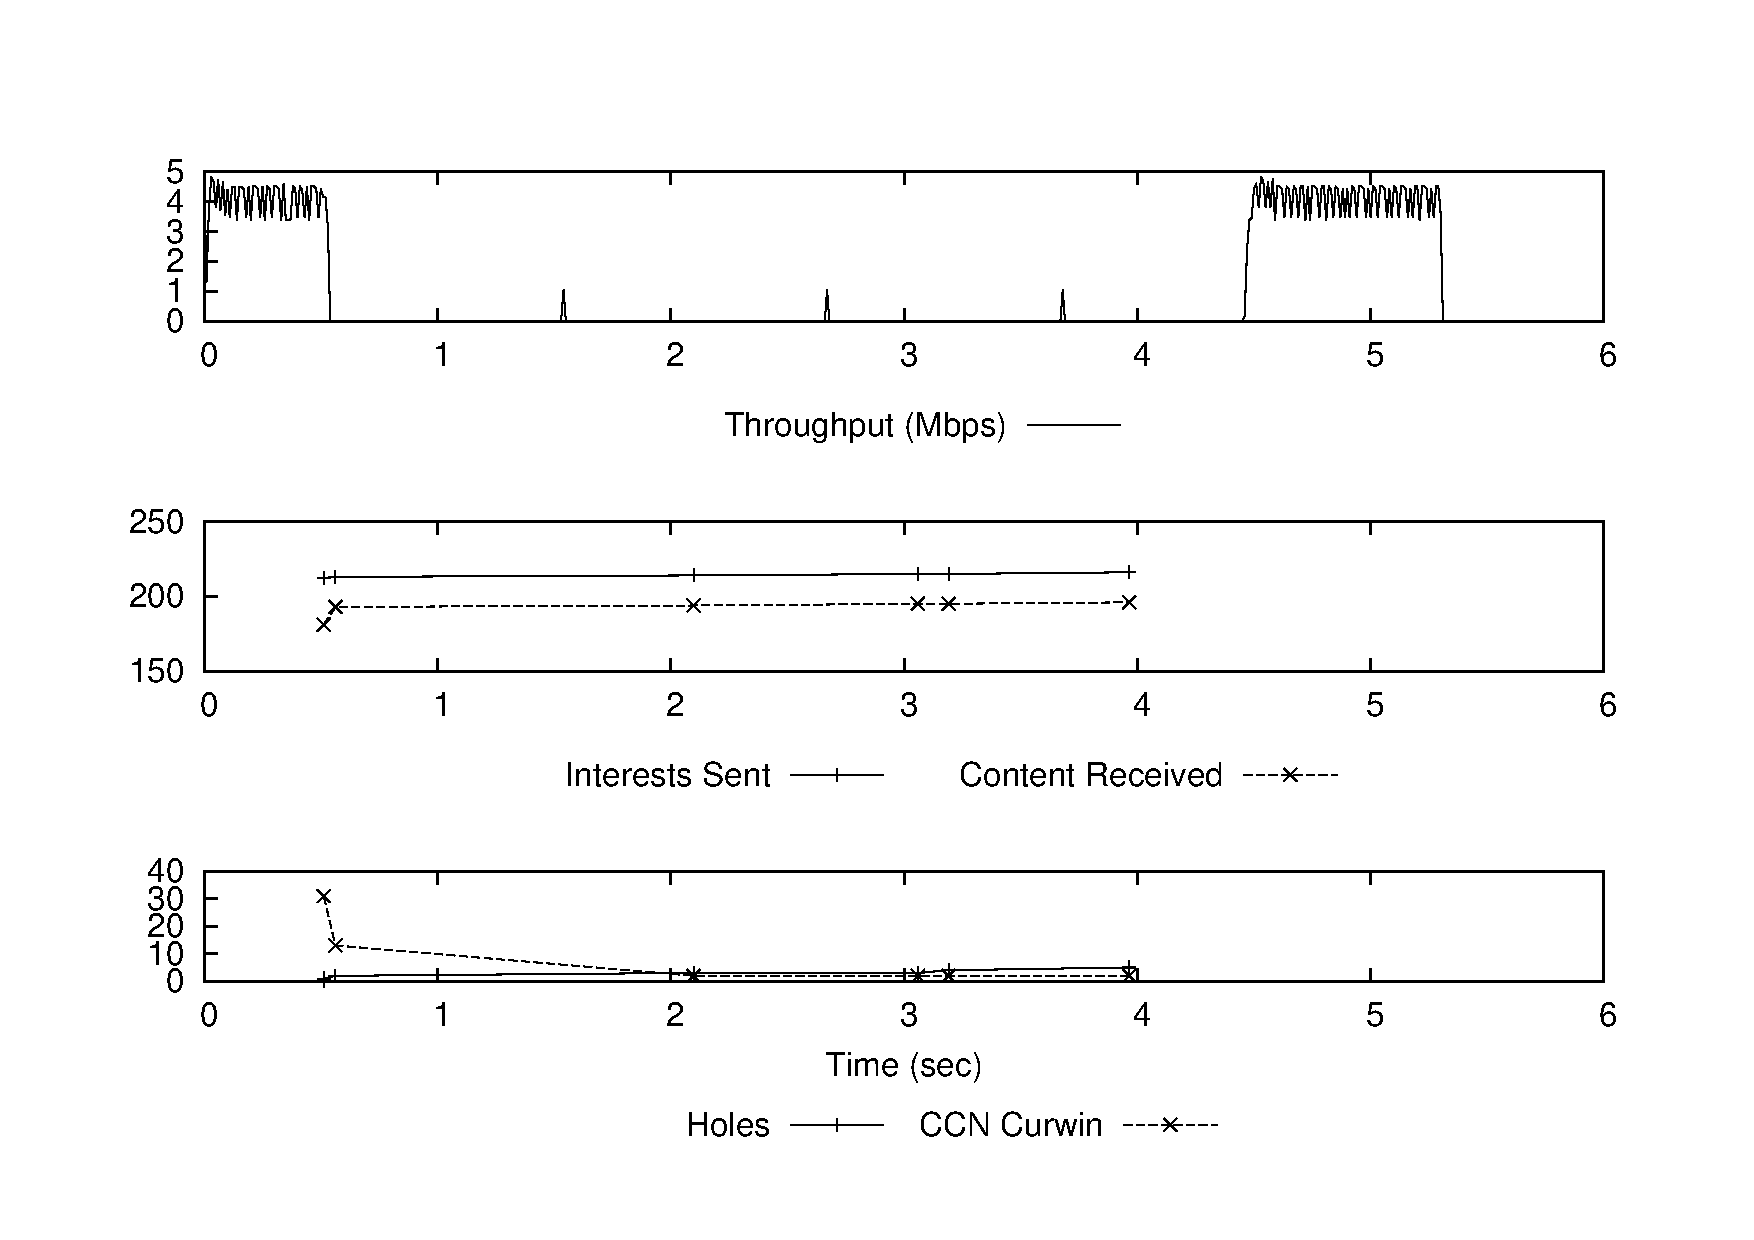
\includegraphics[width=0.75\textwidth]{figures/udp_0_5_1024.pdf}
    \cprotect\caption{Results for Test 1: Throughput in Mbps, as perceived by 
        PC1, when retrieving a file of size 500\,kB with a 1024 byte 
        `chunk' size.}
    \label{fig:test-1-thpt-0_5-1024}

\end{figure}

Figure~\ref{fig:test-1-thpt-0_5-1024} shows the results for the throughput and 
other CCNx specific statistics, as perceived by PC1, when retrieving a file of 
size 500\,kB with a 1024 byte `chunk' size. The action of the joint flow 
control mechanism applied by both \verb+ccncatchunks2+ and \verb+ccnsendchunks+ 
applications (introduced in Section~\ref{subsubsection:disseminating-ccnx}) is 
visible: note how after 0.5 seconds of transfer the throughput drops as well as 
the `Curwin' value (i.e. the size of the window\slash pipeline of Interests 
\verb+ccncatchunks2+ sends to \verb+ccnsendchunks+ at a time), which drops 
from 31 (the maximum size) to 1. Note that such an event is coincident with 
the occurrence of `holes', i.e. a lack of Interest-to-Data packet correspondence. 
After this point, small transferring peaks are visible after approx. 1 second 
intervals, once again consistent with the expected behavior of the 
\verb+ccnsendchunks+ application. This flow control mechanism has 
a severe impact on the overall goodput, i.e. the number of useful information 
bits over the total amount of time required for transfer (approx. 5.35 seconds).\vertbreak

\begin{figure}[h!]

    \centering
    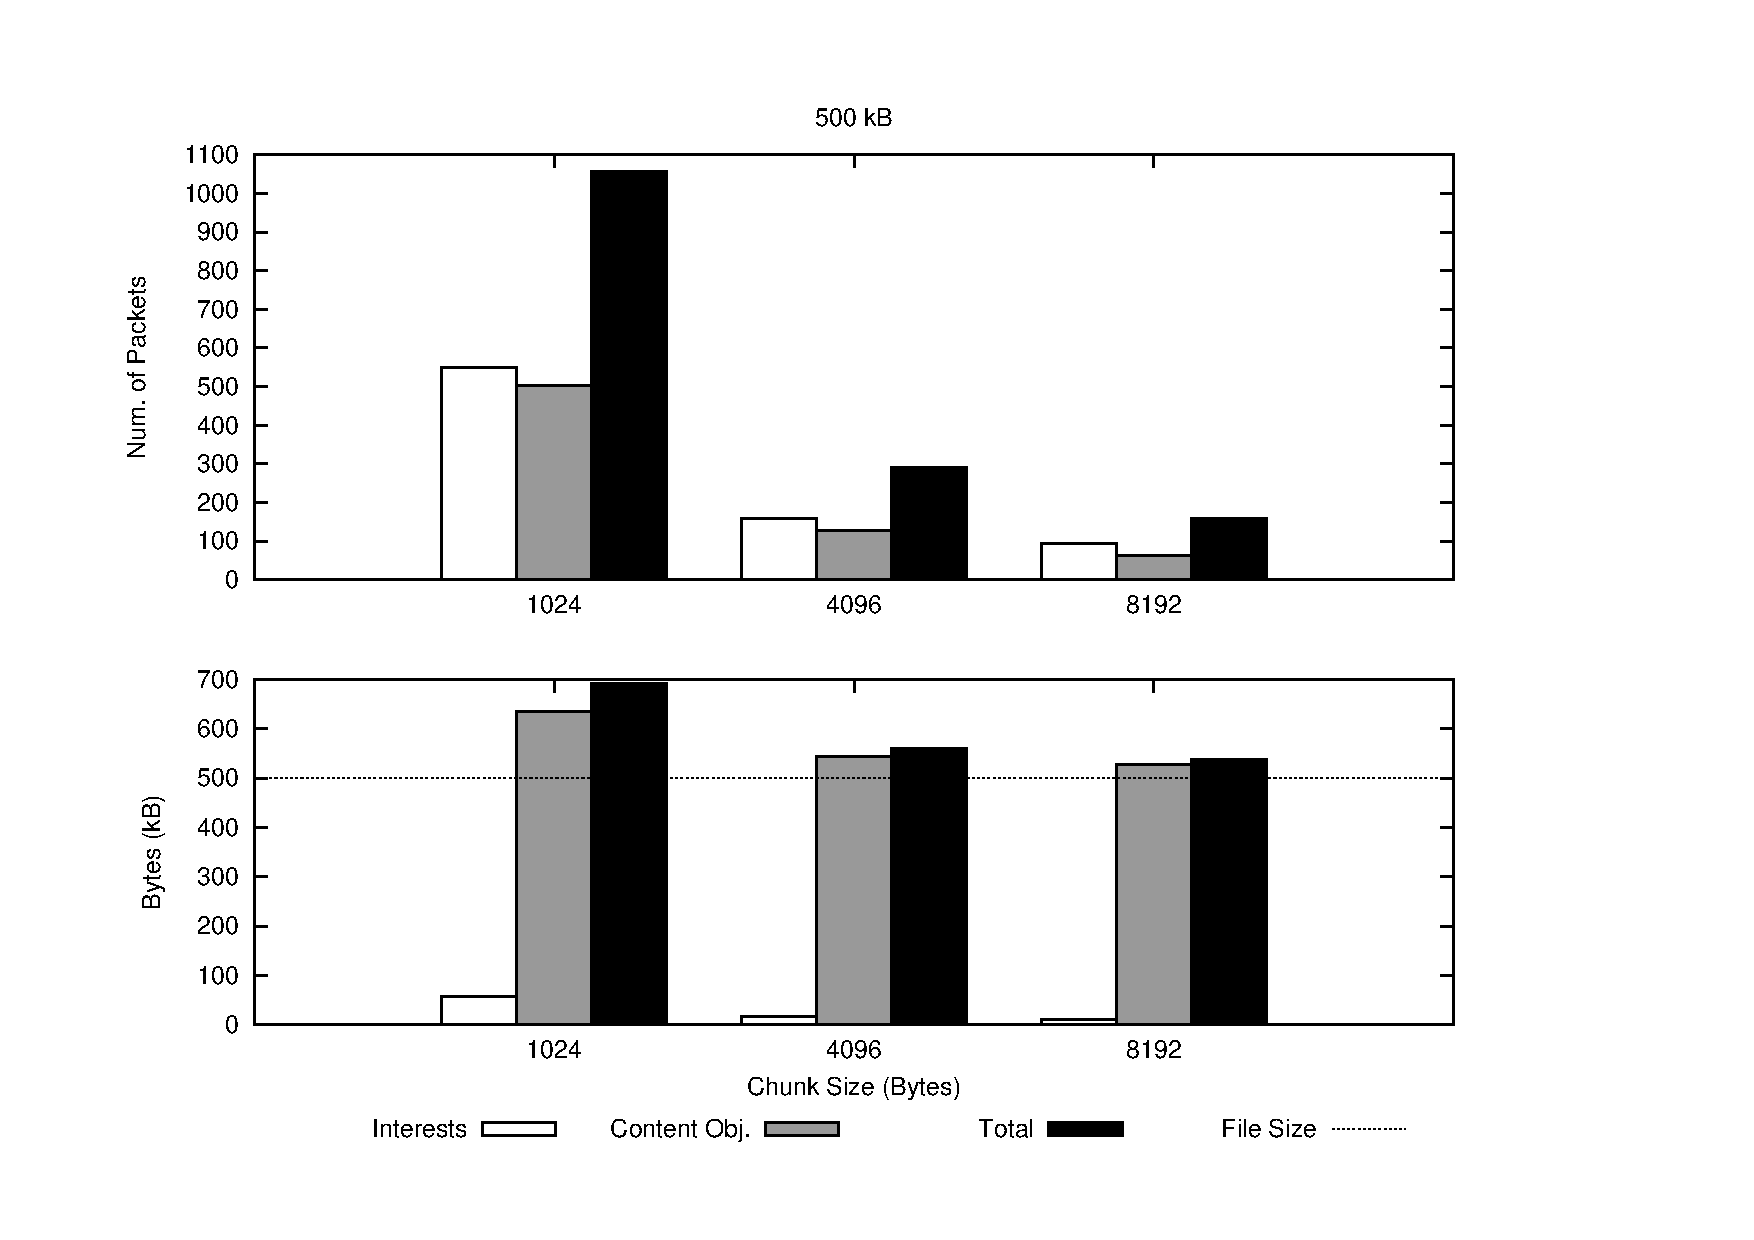
\includegraphics[width=0.75\textwidth]{figures/udp_0_5.pdf}
    \cprotect\caption{Results for Test 1: Packet and byte quantities, measured 
        at PC1, for a file size of 500\,kB.}
    \label{fig:test-1-packtes-bytes}

\end{figure}

Figure~\ref{fig:test-1-packtes-bytes} presents the results for the number of 
packets and bytes, as measured by the capture filters in PC1. Again, we include 
the results for a 500\,kB file size and a `chunk' size of 1024 byte. The amount 
of Interest packets consistently surpasses the amount 
of Data packets, for all `chunk' sizes. This is explained by the 
`loss' of a batch of $N$ pipelined Interest packets, due to overloading of the 
\verb+ccnsendchunks+ application. In the case of 500\,kB, e.g. for a `chunk' 
size of 1024 byte, one can situate the mismatch between Interest and Content 
Objects (or Data packets) within the interval $]0;100]$. This is consistent 
with the results shown in Figure~\ref{fig:test-1-thpt-0_5-1024}, with the 
mismatch being equal to the sum of values of `Curwin', at the time of 
occurrence of `hole' events.\vertbreak

\begin{figure}[h!]

    \centering
    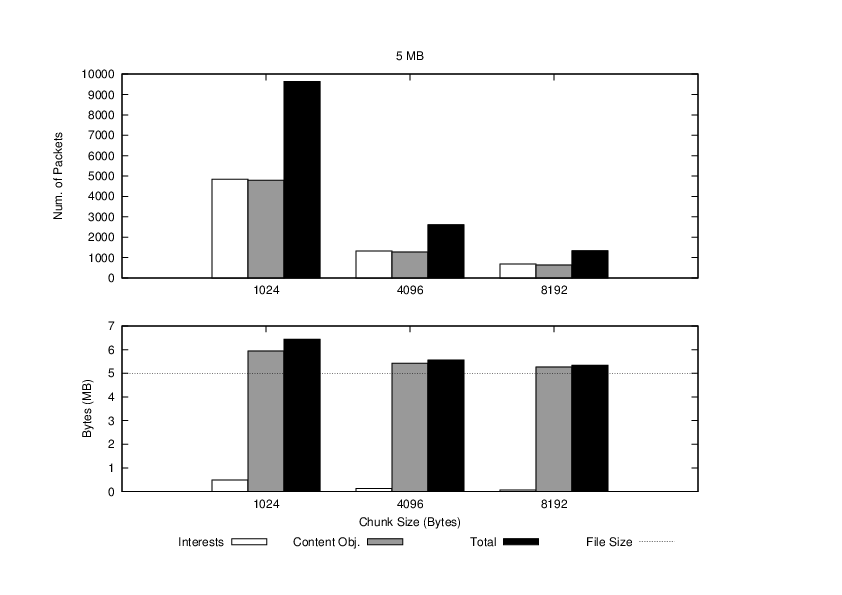
\includegraphics[width=0.75\textwidth]{figures/udp_5.pdf}
    \cprotect\caption{Results for Test 1: Packet and byte quantities, measured 
        at PC1, for a file size of 5\,MB.}
    \label{fig:test-1-packtes-bytes-5}

\end{figure}

\begin{figure}[h!]
    \centering

    \subfigure[]{
        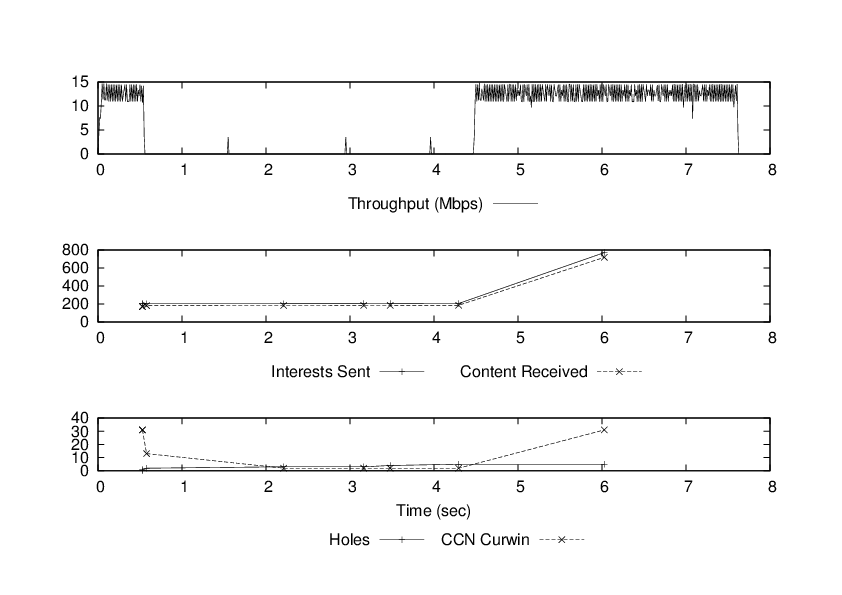
\includegraphics[width=0.75\textwidth] {figures/udp_5_4096.pdf}
        \label{subfig:udp_5_4096}
    }

    \subfigure[]{
        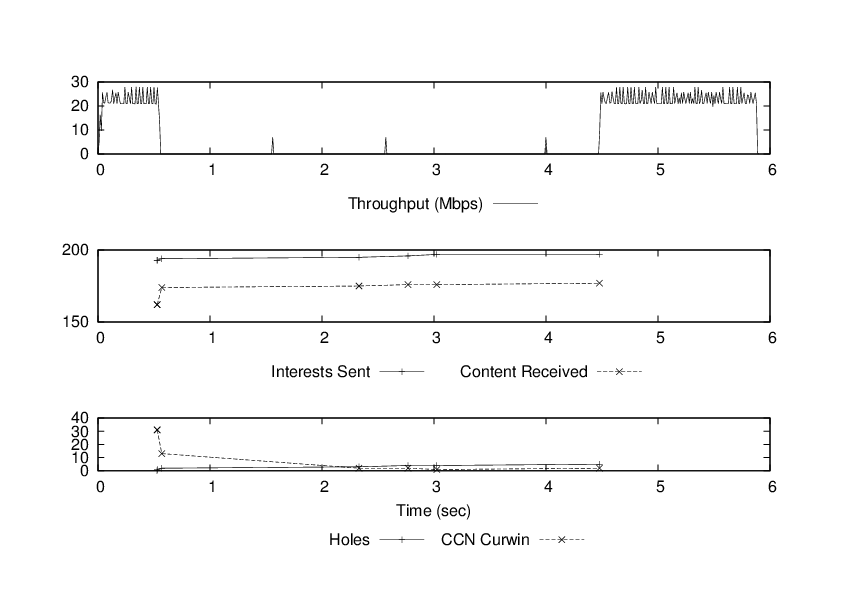
\includegraphics[width=0.75\textwidth] {figures/udp_5_8192.pdf}
        \label{subfig:udp_5_8192}
    }

    \cprotect\caption{Results for Test 1: Throughput in Mbps, as perceived by 
        PC1, when retrieving a file of size 5\,MB with 4096 and 8192 byte 
        `chunk' sizes.}
    \label{fig:udp_5}

\end{figure}

We consider the results for the file size of 5\,MB, depicted in 
Figures~\ref{fig:udp_5} and~\ref{fig:test-1-packtes-bytes-5}, to further 
elaborate on CCNx throughput and overhead. 
In order to easily visualize the impact of the variation of `chunk' size in 
overhead, we have added an horizontal line on the byte quantity charts in 
Figure~\ref{fig:test-1-packtes-bytes-5}, equal to the respective file 
size.\vertbreak 

The difference between the quantity of Content Object bytes and the 
file size decreases as the `chunk' size increases, i.e. the overhead decreases 
with the increase of the chunk size. This can be explained by several 
factors, identified by examining the packet 
capture logs:

\begin{itemize}

    \item The header of a CCNx Content Object, is composed 
        by the following fields (consistent with the Data packet
        descriptions given in Section~\ref{sec:ccn-packets}), resulting in a 
        total max. of 215 byte:

        \begin{enumerate}

            \item Type of packet code (2 byte)
            \item CCN signature (128 byte)
            \item Content name codified as ASCII (32 to 35 byte)
            \item Signed information (50 byte)

        \end{enumerate}

    \item CCNx (at least \verb+ccnsendchunks+ in particular) relies on IP 
        fragmentation to transport Content Object packets with data fields (i.e. 
        payloads) larger than 1480 byte, which is in turn related with the 
        maximum size allowed for a standard Ethernet frame, 1518 byte.

\end{itemize}

So in the case of `chunk' sizes $C$ of 1024 byte, for every 1024 byte of data 
there is an 
additional $~$\,220 byte\,\footnote{By verification of the capture logs, the 
only variable field is the content name, regardless of the `chunk' size.}, while 
in the case of $C = 4096$ or $8192$ byte that header is `spread' over larger 
payload sizes, reducing the overhead. Nevertheless, the overhead of CCNx may 
then be effectively set at 188 byte plus the size of the content name string.\vertbreak

Regarding Figure~\ref{fig:udp_5}, the throughput increases with the 
`chunk' size as well. By verification of the packet capture logs, the throughput 
limitations are imposed by the rate of generation of 
Content Objects and not by the rate at which Interest packets are sent 
(maybe due to the signature generations for each content block 
by part of the \verb+ccnsendchunks+ application\,\footnote{See the discussion 
in \url{https://www.ccnx.org/pipermail/ccnx-dev/2010-April/000188.html}.}), as 
for all file sizes and `chunk' sizes, the average inter-packet arrival times 
for Content Objects (in periods where the throughput is maximum) are 
approximately the same, $\sim$\,2.5 milliseconds. Considering the sizes of 
Content Objects for each 
`chunk' size (including CCNx header), we have the following estimates for 
throughput values, consistent with the values shown in 
Figures~\ref{fig:test-1-thpt-0_5-1024} and~\ref{fig:udp_5}:

\begin{itemize}

    \item 1024 byte: $\frac{1}{0.0025} \times (1024 + 220) \times 8 \approx 3.98$\,Mbps
    \item 4096 byte: $\frac{1}{0.0025} \times (4096 + 220) \times 8 \approx 13.8$\,Mbps
    \item 8192 byte: $\frac{1}{0.0025} \times (8192 + 220) \times 8 \approx 26.9$\,Mbps

\end{itemize}

The results for the non-CCN case, obtained by fetching the same files via FTP 
are shown in Appendix~\ref{app:meas}, in Section~\ref{app:res-throughput-overhead}. As expected, 
the use of channel bandwidth is much more efficient 
(approaching throughput values of Fast Ethernet's 100\,Mbps) as well as lower values of 
overhead. In terms of packet numbers, as FTP avoids payload sizes larger than 
1416 byte (so that frames do not exceed Ethernet’s MTU of 1500 byte), the packet counts 
are (compared with the number of Content Objects) larger.

\section{Test 2 - CCNx Multihop Forwarding}
\label{sec:res-multihop-for}

We now present the results for the CCNx multihop forwarding tests, described 
in Section~\ref{sec:protocol}. We divide the presentation of the results by 
subtype, i.e. the results for Tests 2.1, 2.2 and 2.3 are presented individually.

\subsection{Test 2.1 - CCNx Multihop Forwarding (File Transfer)}
\label{subsec:test-multihop-file-res}

Figure~\ref{fig:file_5-net} depicts the network load (in packets per 
second) at each of the CCNx nodes 
in the testbed (see Figure~\ref{fig:basic-testbed}), for both non-overlapping and 
overlapping file retrieval cases. A 5\,MB file is retrieved via a wireless 
link between CCNx node (IN) CCNx3 and ENs PC1 and PC2. The CCNx 
routes established for this test follow those specified in Figure~\ref{fig:basic-testbed}.\vertbreak

\begin{figure}[h!]
    \centering

    \subfigure[]{
        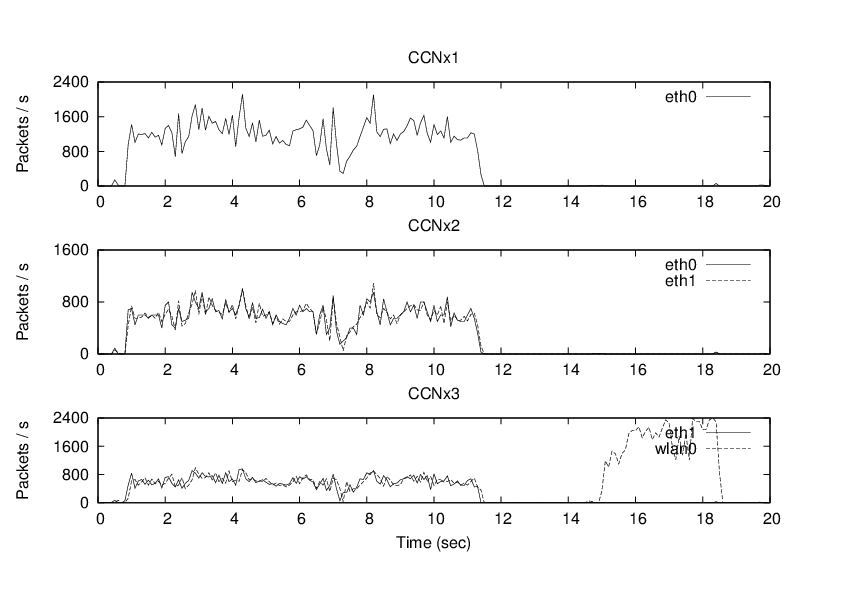
\includegraphics[width=0.75\textwidth] {figures/file_5-sep-net.pdf}
        \label{subfig:file_5-sep-net}
    }

    \subfigure[]{
        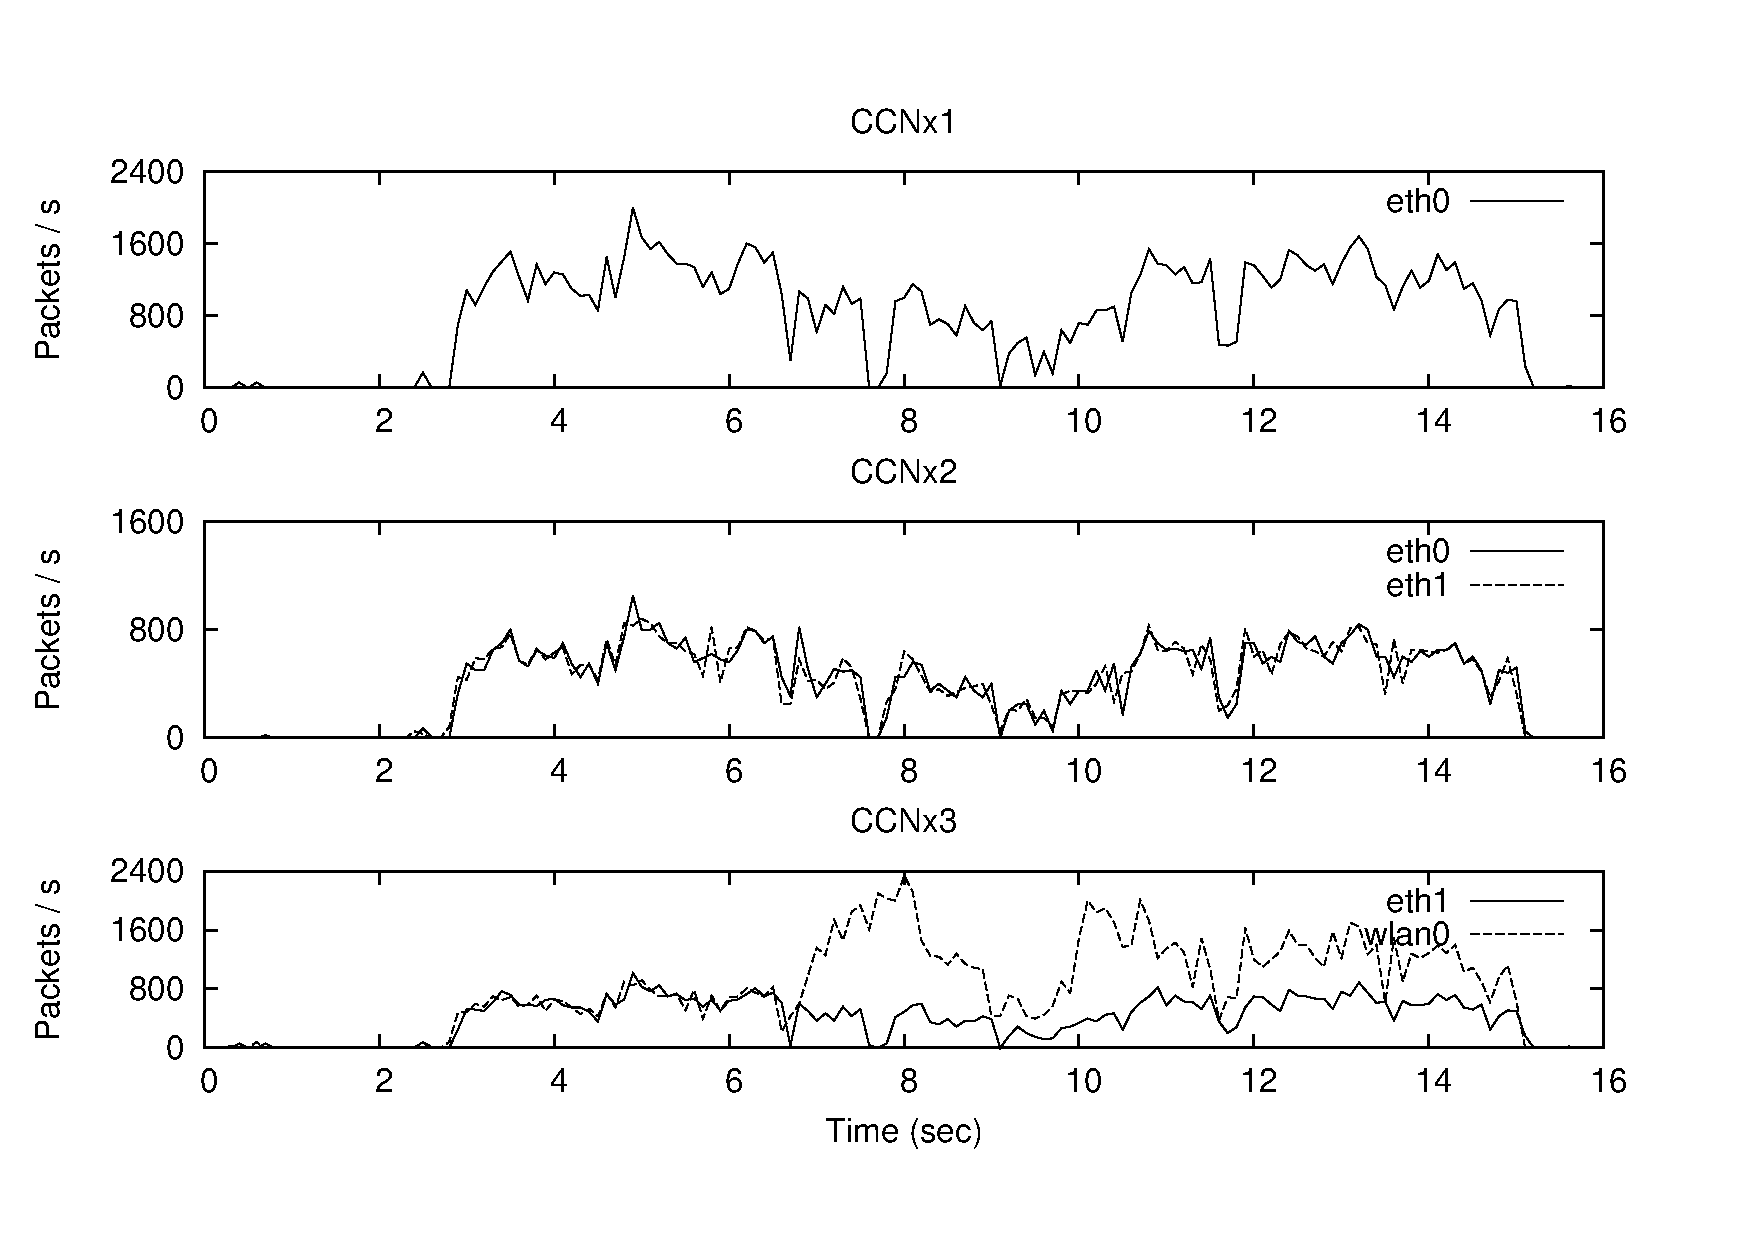
\includegraphics[width=0.75\textwidth] {figures/file_5-sim-net.pdf}
        \label{subfig:file_5-sim-net}
    }

    \cprotect\caption{Results for Test 2.1: Network load, in packets per 
        second, as perceived by each of the CCNx nodes in the testbed, 
        while PC1 and PC2 retrieve a file of size 5\,MB via a wireless 
        link, through CCNx3. The graph in (a) shows the results for 
        the non-overlapping file retrieval, while (b) shows the 
        overlapping case.}
    \label{fig:file_5-net}

\end{figure}

In Figure~\ref{subfig:file_5-sep-net} the effect of CCN's in-network caching 
characteristic is perfectly noticeable: the load on CCNx3 shows two clear 
activity clusters, one for the initial retrieval of the file by PC1, which 
extends for approx. 11 seconds and another for the file retrieval 
by part of PC2, which takes approx. 3 seconds. During the initial period, the 
remaining CCNx nodes display a similar activity pattern, corresponding to 
the forwarding of Interest and Data packets between the several CCNx hops, up 
to the CS node. The values for CCNx1 seem doubled when compared to the other 
nodes, since the forwarding is made via a single interface, \verb+eth0+. The 
second period only shows activity on CCNx1, as expected, as PC2 is 
retrieving the content cached in CCNx1's Content Store. The transfer is 
also clearly faster than in the initial retrieval, as no intermediate CCNx 
forwarders exist between content publisher and subscriber.\vertbreak

In Figure~\ref{subfig:file_5-sim-net}, the load values 
on CCNx3 are similar on both interfaces \verb+eth1+ and \verb+wlan0+, up 
until approx. 7 seconds from the start of the test. At this point, a spike 
on the load for interface \verb+wlan0+ is verified, corresponding to the 
entry of PC2. For an initial period (7 to 8 seconds) PC2 retrieves the 
content already cached at CCNx3, while for the remaining time the Data packets 
arriving at CCNx3 from interface \verb+eth1+ are multicasted to both 
PC1 and PC2. Figure~\ref{fig:file_5-pckt-counts} shows that in terms of 
packet counts --- Interests and Data packets --- there is no difference between 
the overlapping and non-overlapping cases.\vertbreak

\begin{figure}[h!]
    \centering

    \subfigure[]{
        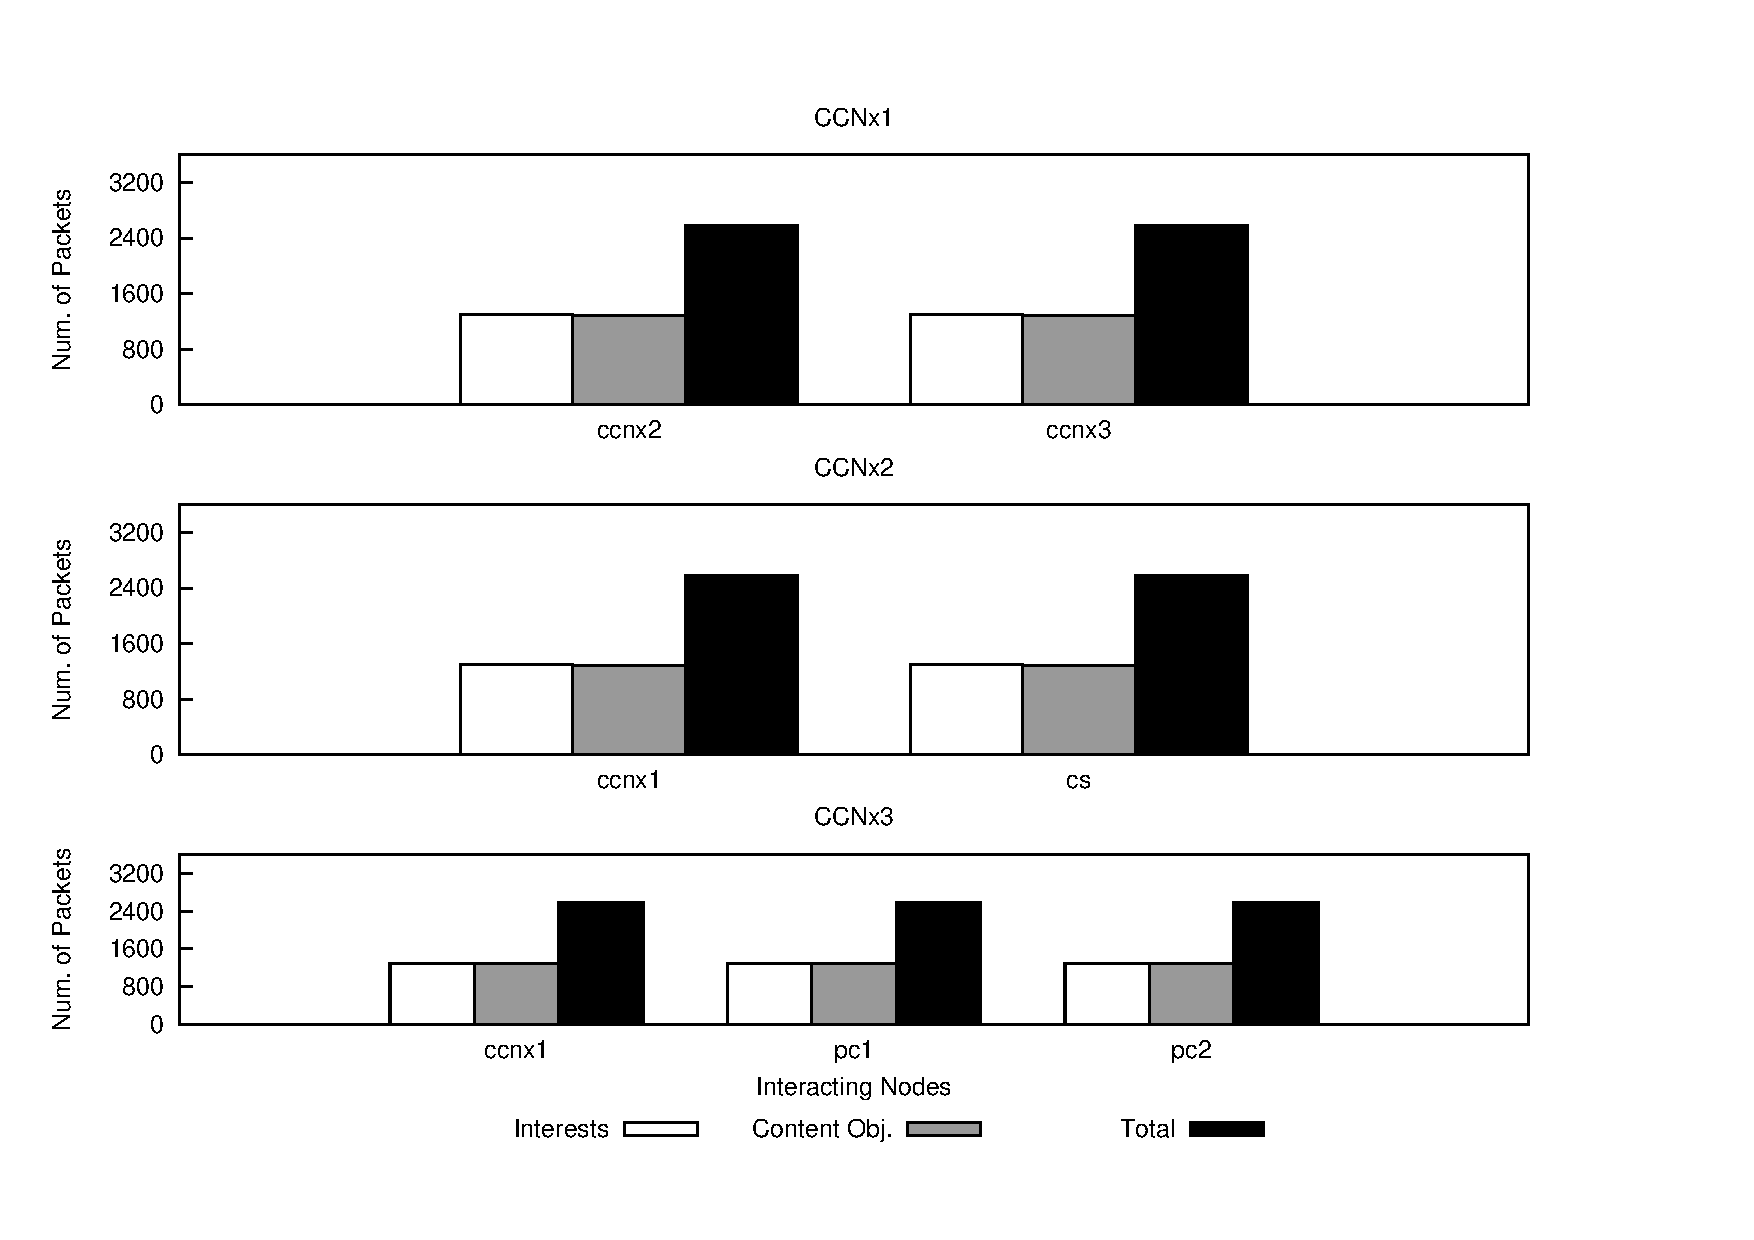
\includegraphics[width=0.75\textwidth] {figures/file_5-sep-pckt.pdf}
        \label{subfig:file_5-sep-pckt}
    }

    \subfigure[]{
        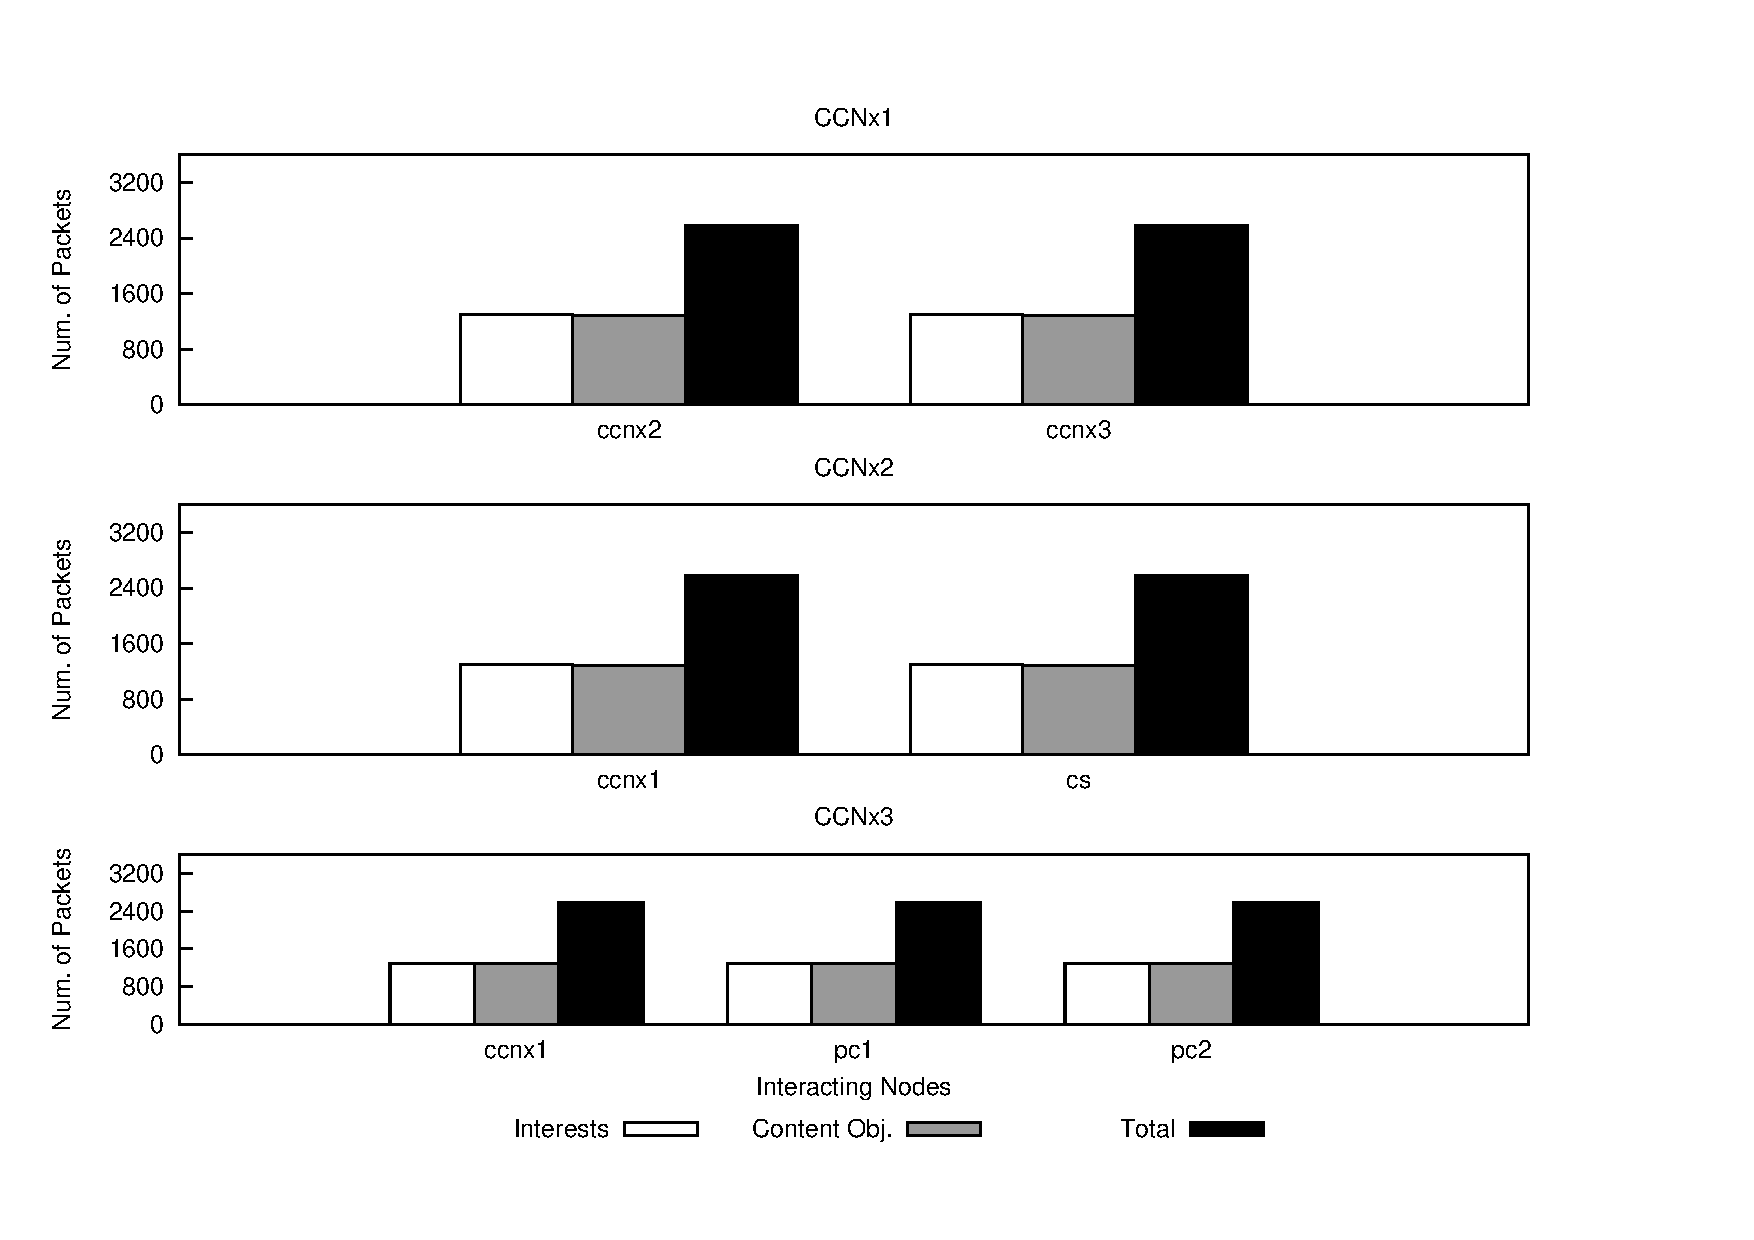
\includegraphics[width=0.75\textwidth] {figures/file-sim-pckt.pdf}
        \label{subfig:file-sim-pckt}
    }

    \cprotect\caption{Results for Test 2.1: Packet counts (Interest and 
        Content Objects) registered at each CCNx forwarding node, exchanged 
        between the respective peer elements. Case (a) presents the results 
        for the non-overlapping case, while (b) shows the results for the 
        overlapping case.}
    \label{fig:file_5-pckt-counts}

\end{figure}

The remaining test cases and results for Test 2.1 can be consulted in 
Appendix~\ref{app:meas}, in Section~\ref{subapp:test-multihop-file}.

\subsection{Test 2.2 - CCNx Multihop Forwarding (Video Streaming)}
\label{subsec:test-multihop-video}

We now present the results for Test 2.2 in Figure~\ref{fig:video-sep-net}. We 
limit the presented results to the network load values at each of the CCNx 
nodes, leaving the remaining measurements to Appendix~\ref{app:meas}.\vertbreak

Similarly to the file transfer results shown in 
Section~\ref{subsec:test-multihop-file-res}, Figure~\ref{subfig:video-sep-net} 
shows two separate network activity clusters: (1) up until approx. 14 seconds 
for the streaming to PC1 and (2) from approx. 17 till 25.5 seconds for the 
streaming to PC2. In terms of time length, (1) clearly exceeds the time 
duration of the video used as sample, which was reflected by several gaps 
in the video playback. In the case of (2) such gaps were still noticed, but 
not as frequent or as long.\vertbreak

\begin{figure}[h!]
    \centering

    \subfigure[]{
        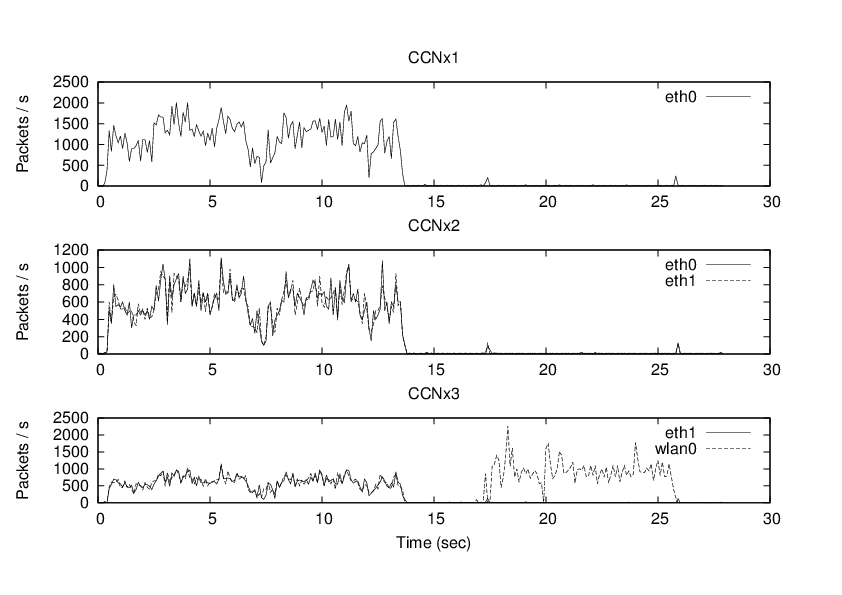
\includegraphics[width=0.75\textwidth] {figures/video-sep-net.pdf}
        \label{subfig:video-sep-net}
    }

    \subfigure[]{
        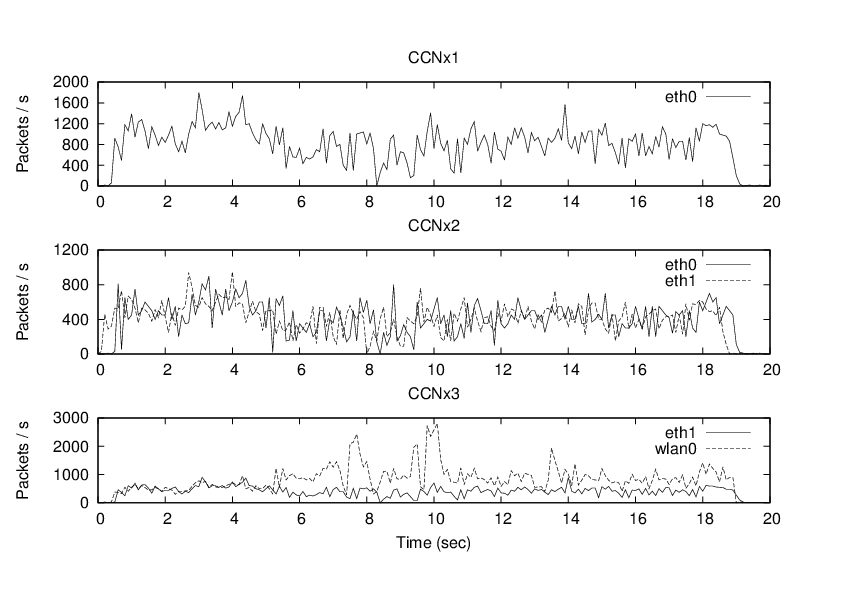
\includegraphics[width=0.75\textwidth] {figures/video-sim-net.pdf}
        \label{subfig:video-sim-net}
    }

    \cprotect\caption{Results for Test 2.2: Network load, in packets per 
        second, as perceived by each of the CCNx nodes in the testbed, 
        while PC1 and PC2 playback a streamed video file of size 6.3\,MB 
        and 8 second duration, via a wireless 
        link, through CCNx3. The graph in (a) shows the results for 
        the non-overlapping streaming case, while (b) shows the 
        overlapping case.}
    \label{fig:video-sep-net}

\end{figure}

In the case of Figure~\ref{subfig:video-sim-net}, again similar results 
to that of Test 2.1 were verified, including a spike in the values of the load 
at CCNx3's \verb+wlan0+ interface upon the initialization of PC2's streaming 
activity, at around 5 seconds after the initialization of the test. Again, the 
time length for the video download is extended, now reflected by frequent gaps 
in the video playback.\vertbreak

\begin{figure}[h!]

    \centering
    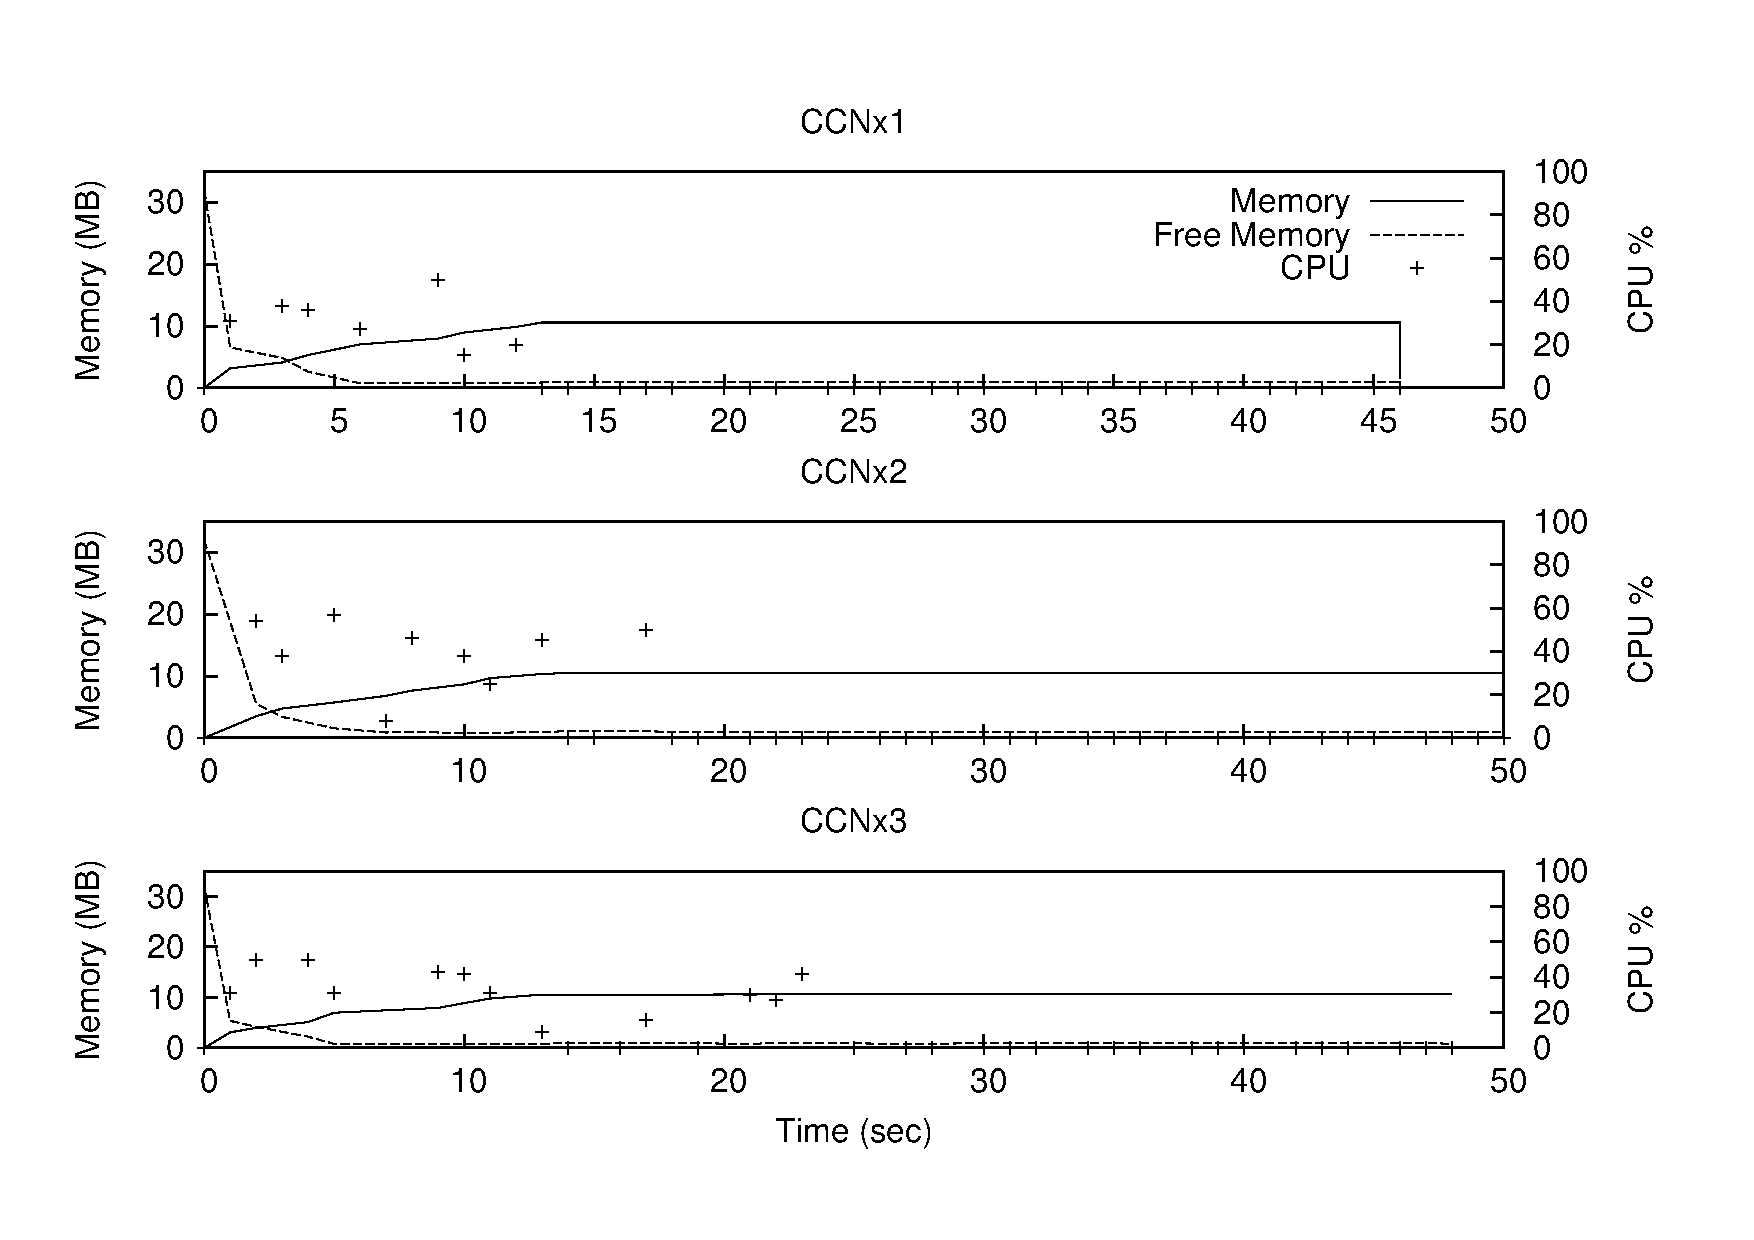
\includegraphics[width=0.75\textwidth]{figures/video-sep-cpu-mem.pdf}
    \cprotect\caption{Results for Test 2.2: CPU and memory utilization at 
        all CCNx nodes, during the streaming of a video file of size 
        6.3\,MB and 8 second duration, non-overlapping case. Regarding the 
        memory values, the `memory' line corresponds to the amount of RAM 
        occupied by the \verb+ccnd+ process, while the `free memory' corresponds 
        to the amount of free memory in the system.}
    \label{fig:video-sep-cpu-mem}

\end{figure}

Figure~\ref{fig:video-sep-cpu-mem} shows the values of CPU and memory 
consumption for the non-overlapping test case. The `memory' line corresponds 
to the amount of RAM used by the CCNx's main process, \verb+ccnd+. It is clear 
how the memory usage increases as the content of the video file is forwarded 
among the CCNx nodes, stabilizing at approx. 14 seconds after the test
 initialization, at the same time the transfer with PC1 is finished. Even though 
these measurements evaluate more the implementation of CCNx than the 
CCN concept itself, these highlight a need for efficient cache 
replacement policies and CCNx applications for constrained devices such as 
the routers used in this experiment. Although for general use cases, CCN nodes 
such as home gateways may have caching disabled, for experimental applications 
such as CCNx applied to Vehicular Networks (VANETS)~\cite{Amadeo2013,Grassi2013}, these 
concerns should be taken into account.

\subsection{Test 2.3 - CCNx Multihop Forwarding (Multiple Paths)}
\label{subsec:test-multihop-multipath}

In the case of the multiple path scenario presented in 
Section~\ref{subsec:mult-path}, we show the results for the packet counts 
registered at each CCNx forwarding node, as the load values are similar to 
those of the non-overlapping version of Test 2.1. Other measurements not 
shown here may be consulted in Appendix~\ref{app:meas}, 
Section~\ref{subapp:test-multihop-multipath}.\vertbreak

Figure~\ref{subfig:long-route} shows the packet counts (Interest and 
Content Objects) registered at each CCNx forwarding node, exchanged 
between the respective peer elements, in this case for the `long' route 
only.\vertbreak 

A note should be 
made to help distinguish the origin of Interest and Content Object packets in the 
chart, which is related to the way the routes are established among 
nodes (see Figure~\ref{fig:testbed-multiple-paths}): e.g. for CCNx1 the value 
of Interest packets associated with `PC1' and `PC2' represents those 
\textit{received} from PC1 and PC2, while the quantity associated with `CCNx3' 
represents the number of Interests \textit{forwarded} to CCNx3. The same 
reasoning can be applied to the Content Objects: those associated with 
`PC1' and `PC2' are \textit{forwarded} to these nodes, while the values associated 
with `CCNx3' correspond to the Content Objects \textit{received} from CCNx3.\vertbreak

The values in Figure~\ref{subfig:long-route} are expected, with no 
divergences between the number of forwarded packets between each of the 
INs and ENs. Furthermore, the existence of a single path (or 
conversely the absence of the `short' path) is noticed by the 
absence of values associated with CCNx2 and CCNx1 for nodes CCNx1 and CCNx2, 
respectively.\vertbreak

\begin{figure}[h!]
    \centering

    \subfigure[]{
        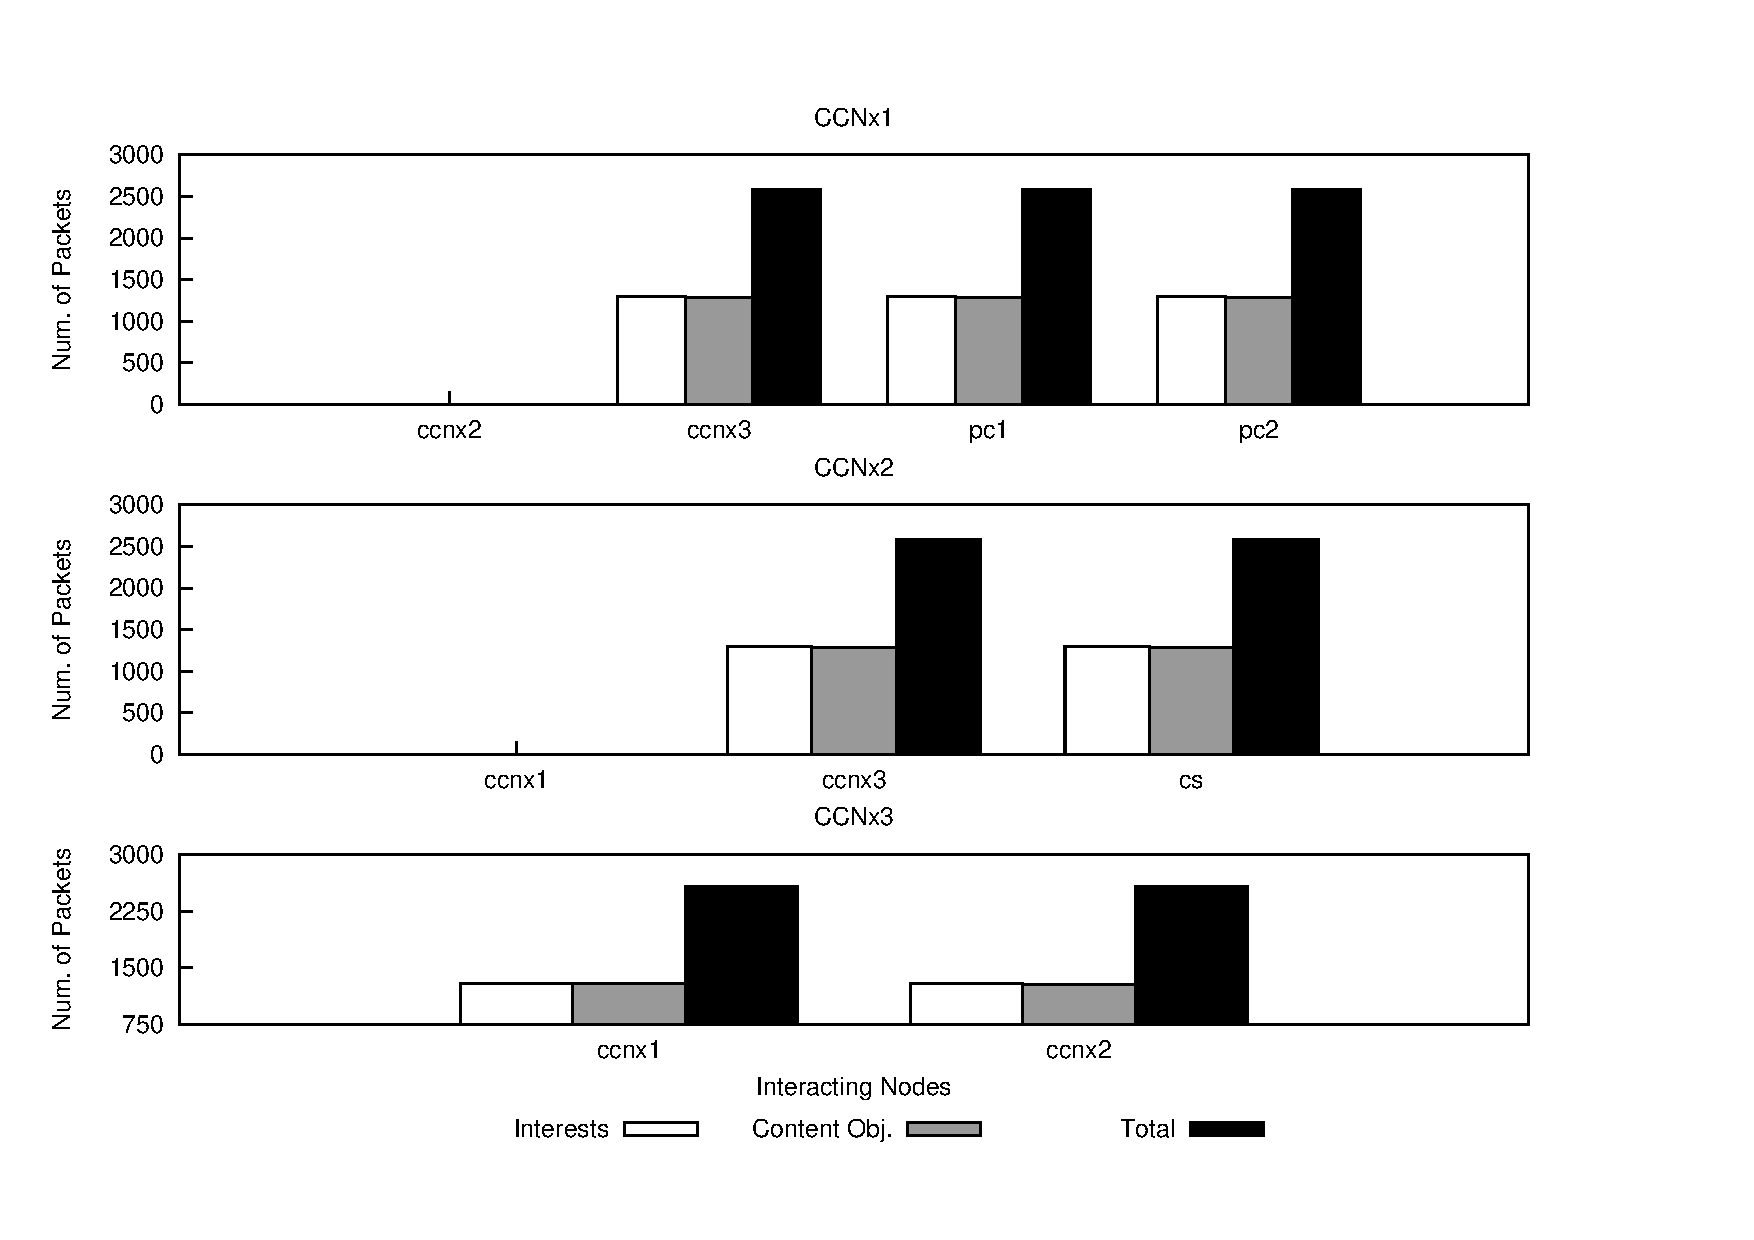
\includegraphics[width=0.75\textwidth] {figures/long-route.pdf}
        \label{subfig:long-route}
    }

    \subfigure[]{
        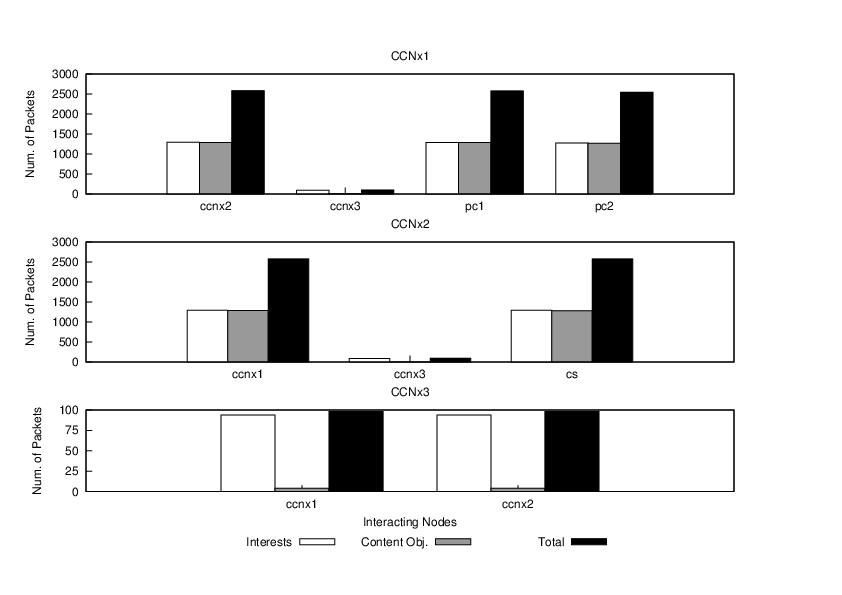
\includegraphics[width=0.75\textwidth] {figures/long-short-route.pdf}
        \label{subfig:long-short-route}
    }

    \cprotect\caption{Results for Test 2.3: Packet counts (Interest and 
        Content Objects) registered at each CCNx forwarding node, exchanged 
        between the respective peer elements. Case (a) presents the results 
        for the `long' route only, while (b) shows the results for multiple 
        paths, i.e. with the junction of both `long' and `short' routes.}
    \label{fig:routes-pckt-counts}

\end{figure}

In the case of Figure~\ref{subfig:long-short-route}, the presence of multiple 
paths is visible by the amount of Interest packets which are forwarded along 
the `long' path, i.e. from CCNx1 to CCNx3 and then from CCNx3 to CCNx2. From 
consultation of the capture logs, one verifies that a small quantity of 
Interest packets ($\sim 90$) is forwarded by CCNx1 to both CCNx2 and CCNx3. 
Only a residual number of Content Objects is forwarded by 
CCNx2 to CCNx3, corresponding to special CCNx packets exchanged among peers, 
not directly related to the content being requested by PC1 and PC2 (these 
pertain to `probing' Interest packets, periodically sent along alternative 
interfaces in order to detect better paths~\cite{Yi2013}). As the 
Interests forwarded by CCNx3 to CCNx2 are duplicated (arriving after those 
issued by CCNx1), these are discarded by CCNx2.

